\documentclass[10pt, xcolor=table]{beamer}

\setbeamertemplate{note page}[default]
\setbeameroption{hide notes}
%\setbeameroption{show notes}
\setbeamerfont{footnote}{size=\tiny}

\usetheme[progressbar=frametitle]{metropolis}
\usepackage{appendixnumberbeamer}

\usepackage{booktabs}
\usepackage[scale=2]{ccicons}

\usepackage{pgfplots}
\usepgfplotslibrary{dateplot}
\usepackage{multicol}
\setlength{\columnsep}{1.5cm}
\usepackage{multirow}

\usepackage{hyperref}
%\usepackage{animate}
\usepackage{lmodern}
\usepackage[T1]{fontenc}
\usepackage{mathtools}
\usepackage{graphicx}
\usepackage[font=scriptsize]{caption}
\usepackage{tikz}
\usepackage{stackengine}
\usepackage{array}
\usetikzlibrary{positioning}
\usepackage{tabularx}
\usepackage{tabulary}
%\hypersetup{
%    colorlinks=true,
%    linktoc=none,
%    linkcolor=blue,
%    urlcolor=blue
%}

\usepackage[math]{cellspace}
\cellspacetoplimit 2pt
\cellspacebottomlimit 2pt


%\definecolor{set1}{RGB}{228, 26, 28}
%\definecolor{set2}{RGB}{77, 175, 74}
%\definecolor{set3}{RGB}{255, 127, 0}
%\definecolor{set4}{RGB}{166, 86, 40}
%\definecolor{set5}{RGB}{153, 153, 153}

\usepackage{xspace}
\newcommand{\themename}{\textbf{\textsc{metropolis}}\xspace}

\newcommand\Fontvi{\fontsize{8}{9}\selectfont}
\newcommand\Fontvr{\fontsize{6}{7}\selectfont}

\setbeamerfont{parent A}{size=\small}

\DeclarePairedDelimiter\abs{\lvert}{\rvert}%
\DeclarePairedDelimiter\norm{\lVert}{\rVert}%
\makeatletter
\let\oldabs\abs
\def\abs{\@ifstar{\oldabs}{\oldabs*}}
\let\oldnorm\norm
\def\norm{\@ifstar{\oldnorm}{\oldnorm*}}
\makeatother
\newcommand*{\Value}{\frac{1}{2}x^2}%

\newcommand{\floatfootnote}[1]{\ifx\[$\else\footnote{#1}\fi}
\newcommand{\floatfootnotes}[1]{\ifx\[$\else\footnote{#1}\fi}



\title{Digital Transformation of Healthcare}
\subtitle{Data Cleaning}
% \date{\today}
\date{}
\author{Michoel Snow, M.D. Ph.D., Glen Ferguson, Ph.D.}
\institute{Center for Health Data Innovations}
% \titlegraphic{\hfill\includegraphics[height=1.5cm]{logo.pdf}}

\begin{document}

\maketitle


\begin{frame}{Data Cleaning}
	After this lecture students will be able to 
	\begin{itemize}
		\item Discuss and apply the steps involved in cleaning data for modeling
		\item Design a process for the imputation of missing data 
		\item Build a bioinformatics pipeline starting from given data
	\end{itemize}
\end{frame}


\begin{frame}{Bioinformatics Pipeline}
	\begin{center}
		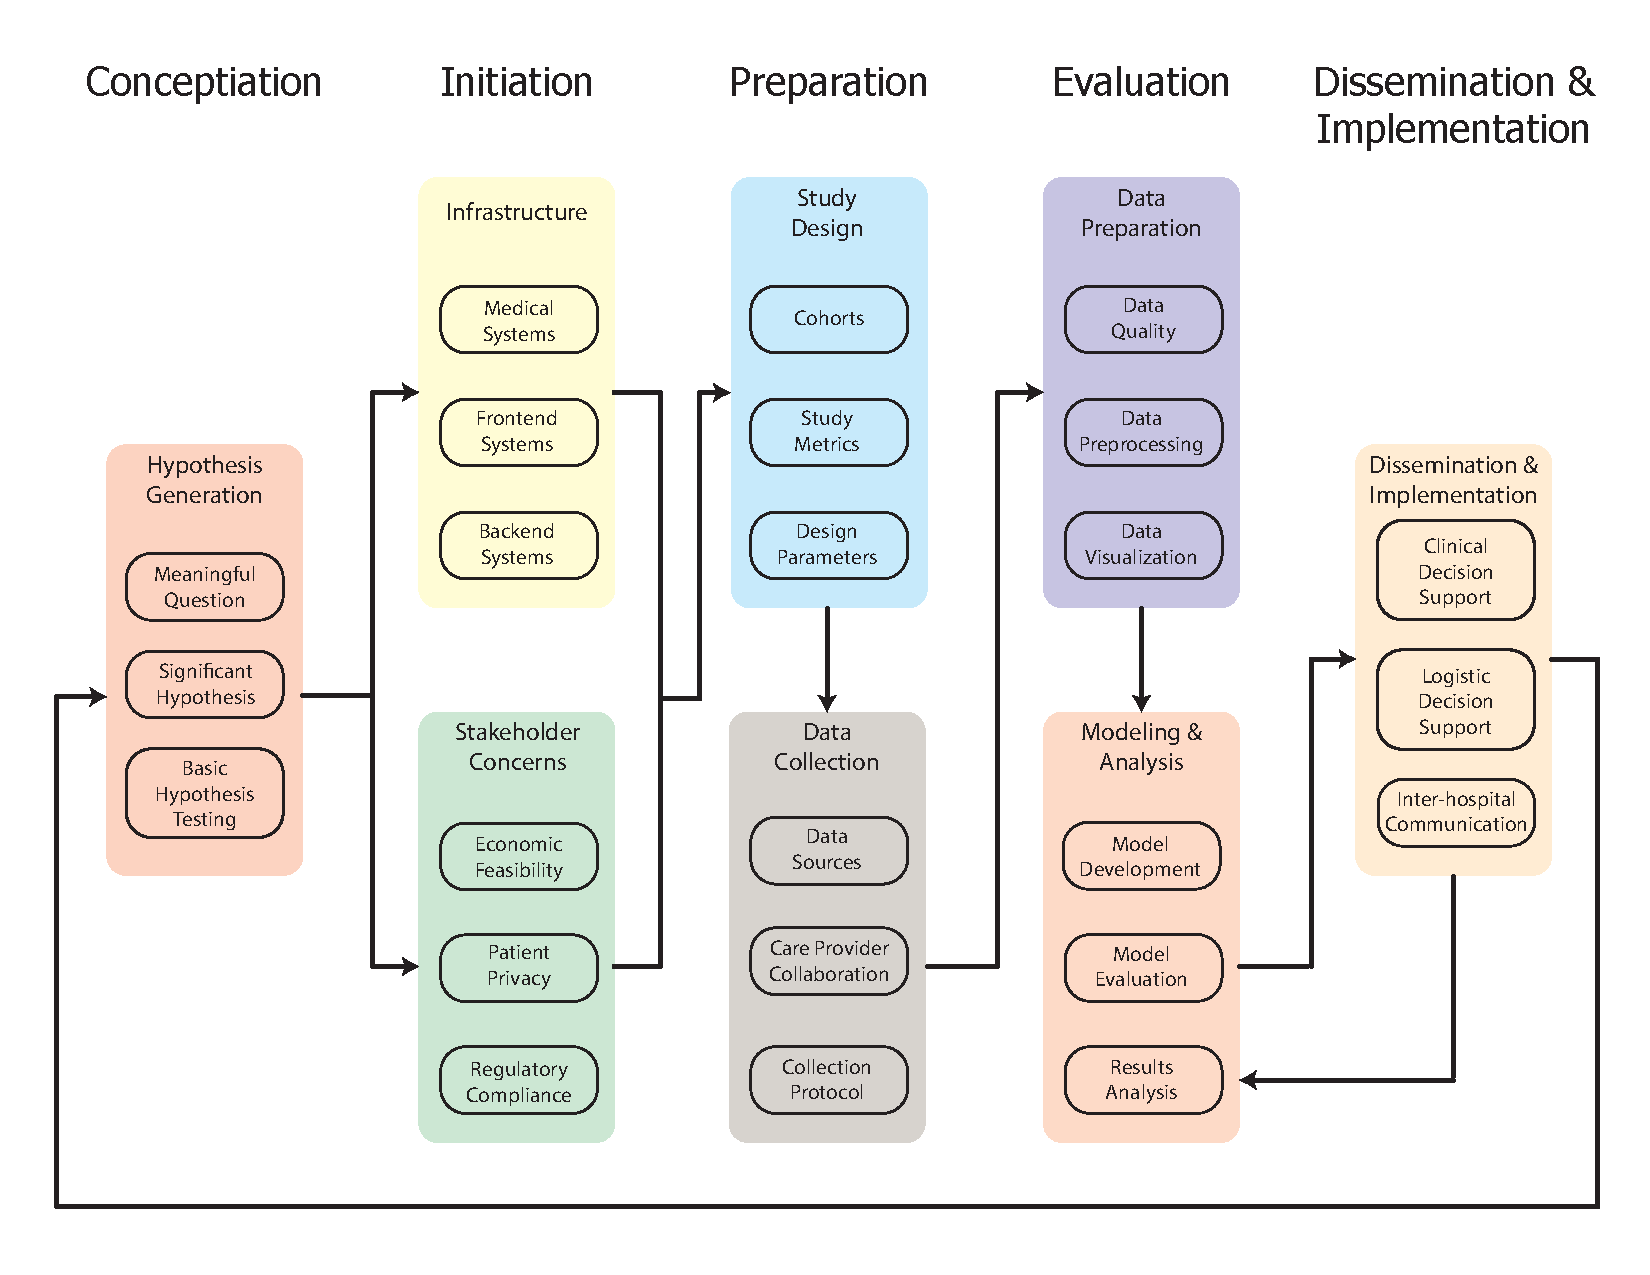
\includegraphics[width=0.9\textwidth]{images/informatics_pipeline.pdf}	
	\end{center}
\end{frame}


\begin{frame}{Data Cleaning}
	\begin{center}
		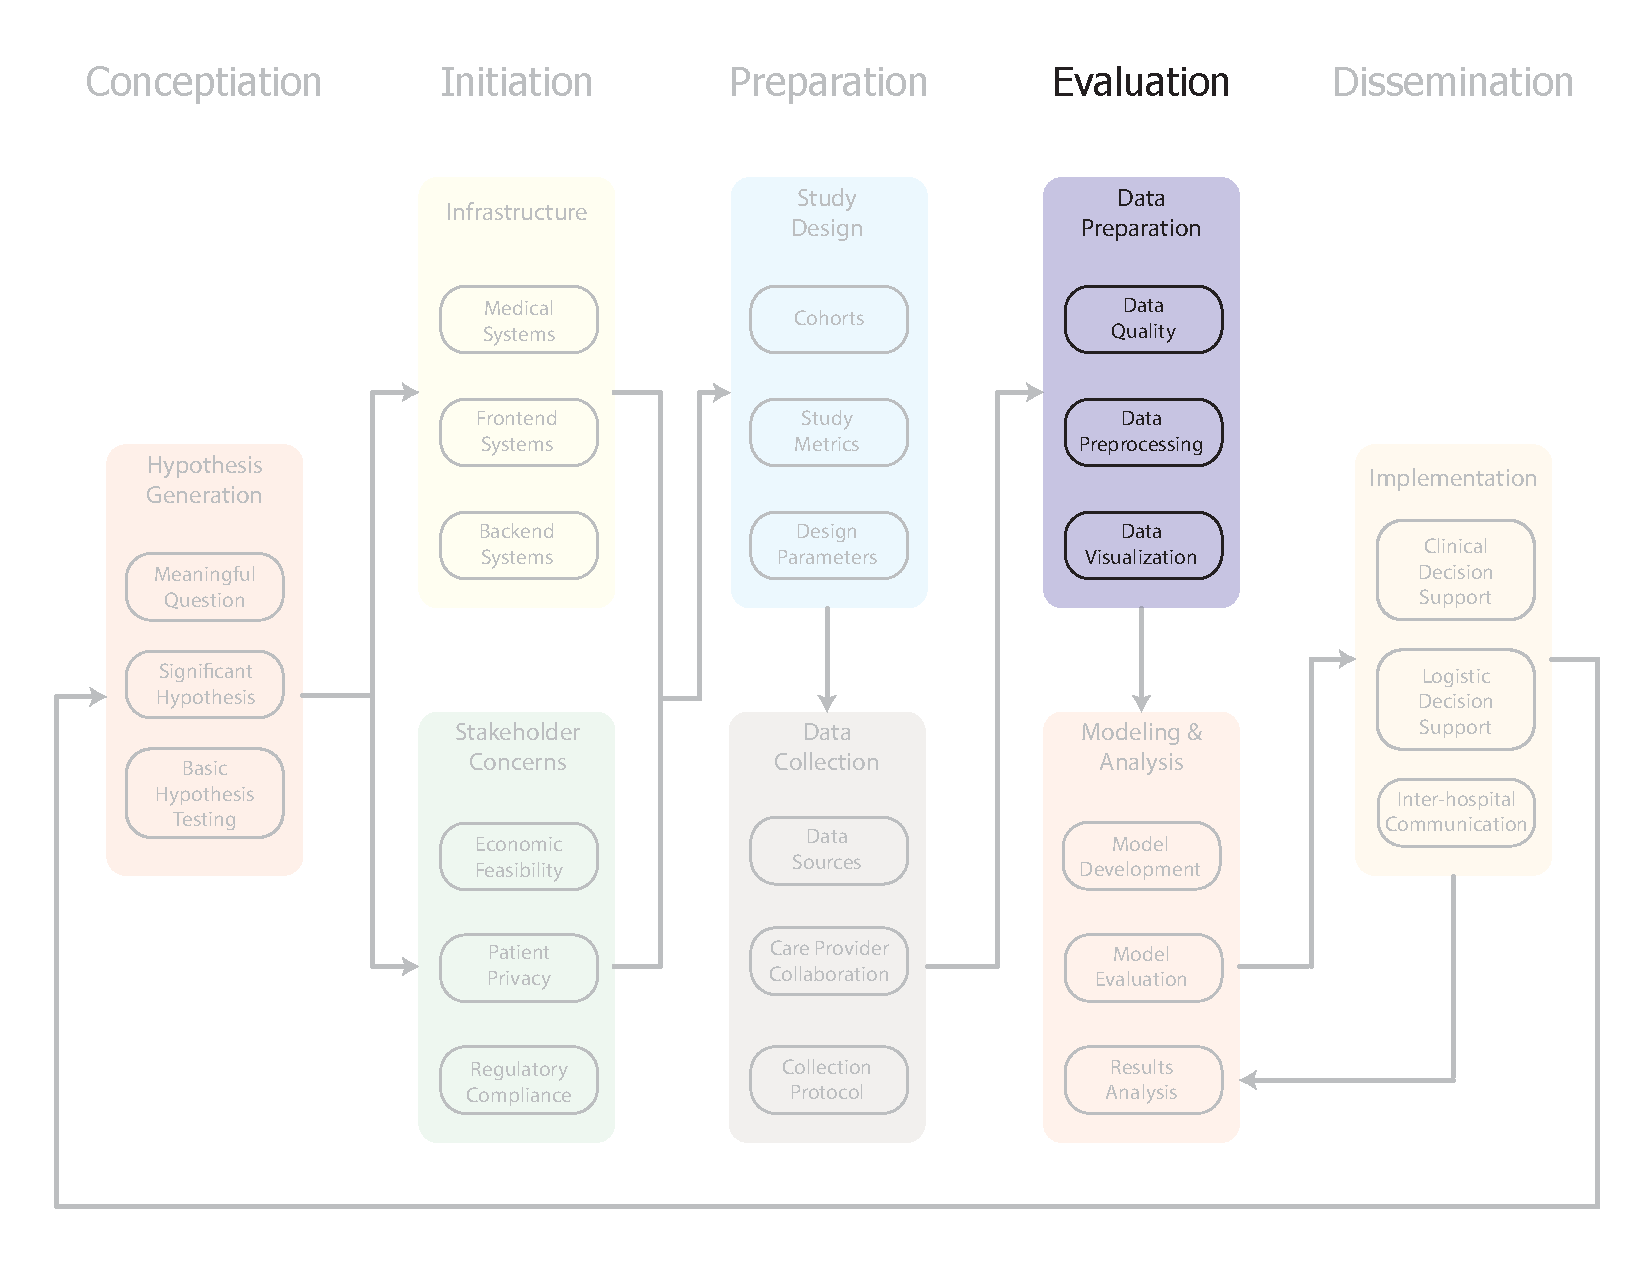
\includegraphics[width=0.9\textwidth]{images/informatics_pipeline_data_quality.pdf}	
	\end{center}
\end{frame}


\begin{frame}{Scenario}
	\begin{itemize}
		\item You are trying to optimize the use of pain medication regimens for pediatric sickle cell patients
		\item You have just collected all the data on all peds hem-onc patients on the floor for the past month.
		\item How can you systematically assess, organize and prepare the data for modeling and analysis? 
		\begin{itemize}
			\item What are the steps to transform raw data into a usable format
		\end{itemize}
	\end{itemize}
	\begin{center}
		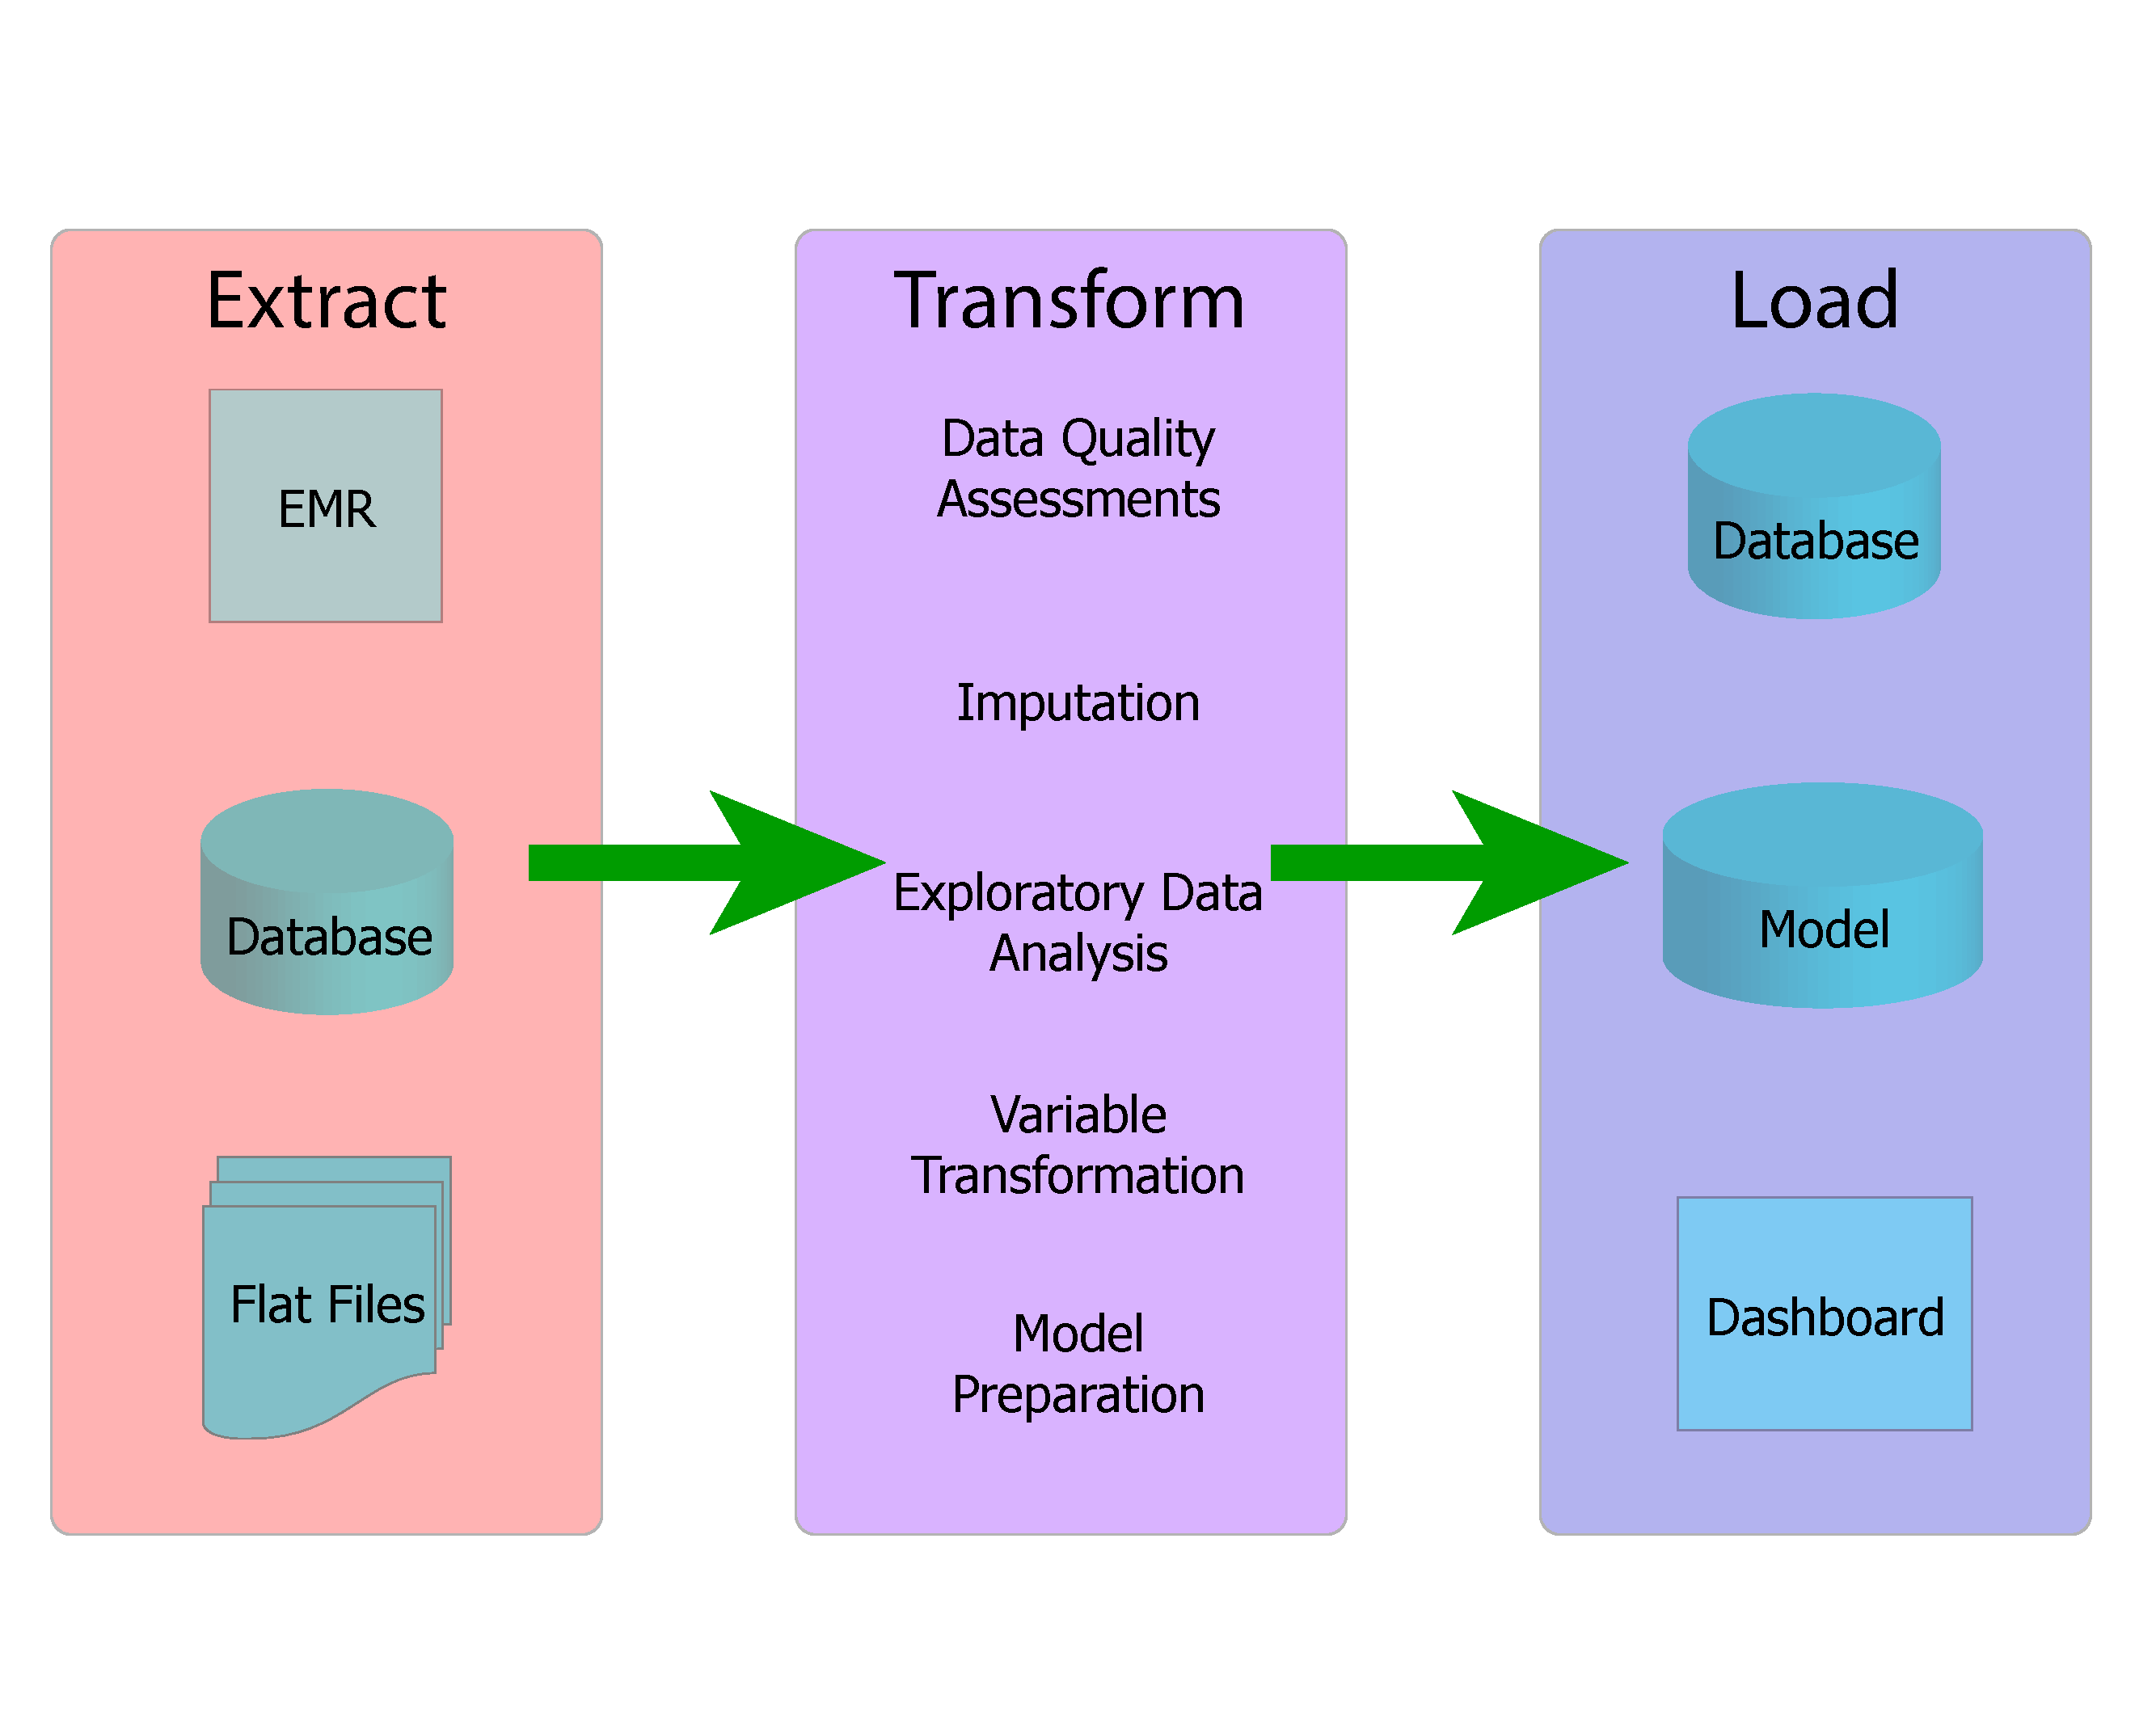
\includegraphics[width=0.5\textwidth]{images/etl.pdf}	
	\end{center}
\end{frame}

\note{
	\scriptsize
	\begin{itemize}
		\item Data encoding
		\item variable correctness, i.e., what percentage of the data is missing (and does that percentage make sense (birth date vs death date), are all the values the same
		\item variable quality
		\item Data organization/ time frequencies - Ensure that time blocks used in time series data are appropriate to the task (Do you need to group your data or can they all be left as individual data points, e.g., do I want to know all of my patient's lab values every 6 hours, or can I take them as they come in.  Loaf of bread model vs streaming model.)
		\item drop corrupt data, variables and time blocks
		\item impute and/or mask missing variables
	\end{itemize}

}



\begin{frame}{Imputation and Extrapolation}
	\begin{itemize}
		\item what are the different reasons why data might be missing
		\item What are the different ways that data could be missing
		\item Can we develop a systematic way to deal with missing data
		\begin{itemize}
			\item pain score
			\item pain medication usages
			\item retic count
			\item infection status
			\item imaging results
		\end{itemize}
		\item How do you evaluate imputation
	\end{itemize}
\end{frame}

\note{
	\scriptsize
	\begin{itemize}
		\item data could be mcar, mar (dependent on an observed variable, which can be controlled for), mnar or because we are slicing the data into chunks smaller than the sampling rate or there is no value, e.g., death date for a living patient
		\begin{itemize}
			\scriptsize
			\item How is the data missing, e.g., first values, random values, ...
			\item when is there too much missing data
			\item correlation/heatmap of missingness 
		\end{itemize}
		\begin{itemize}
			\scriptsize
			\item categorical fill, cases where missingness tells you information e.g., missing date of x-ray could be another class in that column, as empty but not missing
			\item ffill, mean fill, back fill
			\item drop blocks if data is bad or empty
			\item Drop beginning blocks if empty, drop end blocks if dead or discharged
			\item \textbf{Imputation} - MICE, NN, KNN
			\item  Anything which is not imputed is masked (-9999, not 0)
		\end{itemize}
		\item check through hand created missingness accuracy as well as downstream calculations
	\end{itemize}
}


%\note{
%	\scriptsize
%	\begin{itemize}
%		\item data could be MCAR, MAR (dependent on an observed variable, which can be controlled for), MNAR or because we are slicing the data into chunks smaller than the sampling rate or there is no value, e.g., death date for a living patient
%		\item Missing Data Procedure
%		\begin{itemize}
%			\scriptsize
%			\item \textbf{Variable correctness} -  
%var correctly derived/appropriate to include, e.g., complete or near-complete missingness or same value in all rows.
%			\item \textbf{Time freq} - Ensure that time blocks used in time series data are appropriate to the task
%			\item Determine how frequently every variable is measured
%			\item Use the frequency range from the previous step for each variable to do ffill
%			\item Encounters without data or good data cannot add value and should be dropped.
%			\item Drop beginning blocks if empty, drop end blocks if dead or discharged
%			\item \textbf{Imputation} - MICE, NN.  Cases where imputation should not be done are when the missingness itself is significant or if the imputation cannot be done by adding another class.  An example of the latter is would be if an x-ray is performed. X-rays not being performed are another class that can be added to the column.
%			\item  Anything which is not imputed is masked (-9999, not 0)
%		\end{itemize}
%	\end{itemize}
%}

\begin{frame}{Imputation Example}
	\begin{center}
		Missing Data Imputation in the Electronic Health Record Using Deeply Learned Autoencoders
	\end{center}
	\begin{itemize}
		\item Researchers started from an ALS clinical trials database of 10,723 patients
		\item The dataset includes  patient demographic data, family history, concomitant medications, vital sign measurements, laboratory results, and patient clinical history
		\item They removed data using either an MCAR or MNAR approach
		\item For end metrics they considered both accuracy in imputation and ALS functional rating scale
	\end{itemize}
\end{frame}


\begin{frame}{Imputation Example}
	\begin{center}
		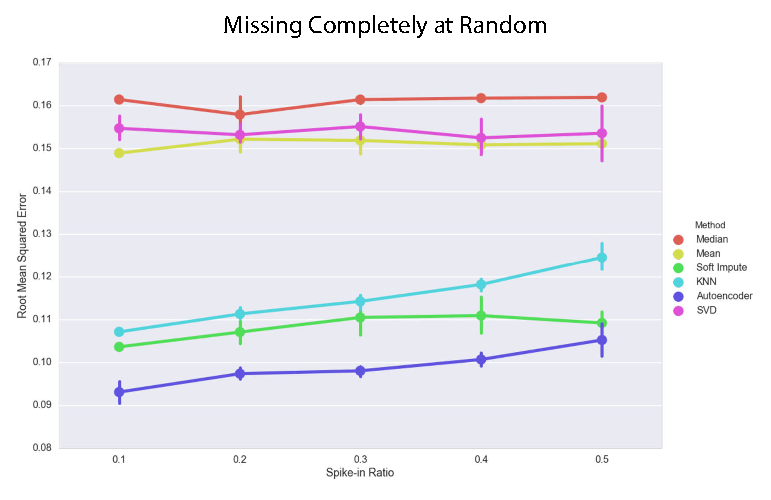
\includegraphics[width=1\textwidth]{images/paper_mcar.pdf}	
	\end{center}
\end{frame}

\begin{frame}{Imputation Example}
	\begin{center}
		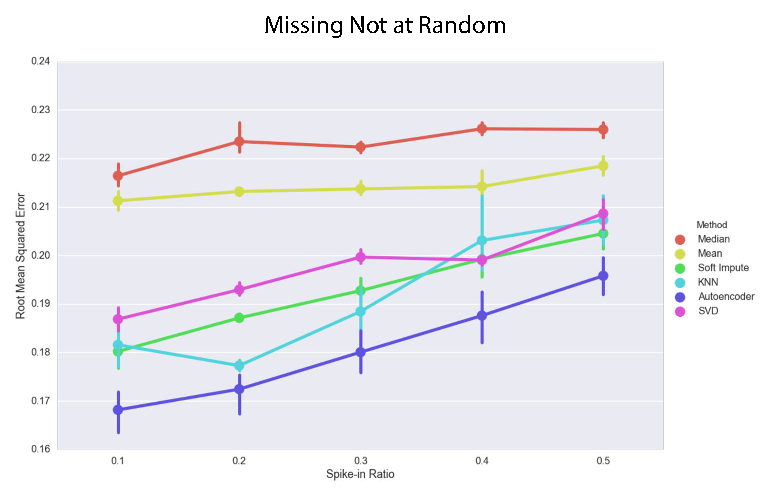
\includegraphics[width=1\textwidth]{images/paper_mnar.pdf}	
	\end{center}
\end{frame}

\begin{frame}{Imputation Example}
	\begin{center}
		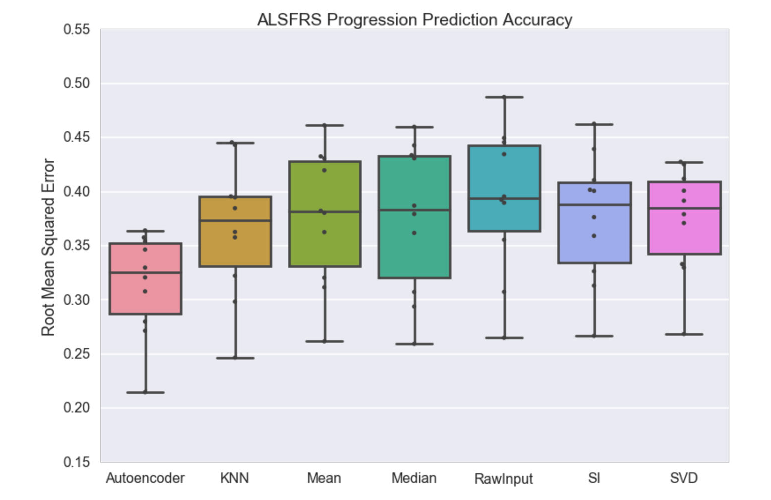
\includegraphics[width=1\textwidth]{images/paper_alsfrs.pdf}	
	\end{center}
\end{frame}


\begin{frame}{Pipeline}
	\begin{itemize}
		\item Using the pediatric sickle cell example let's walk through building the second half of the bioinformatics pipeline
	\end{itemize}
	\begin{center}
		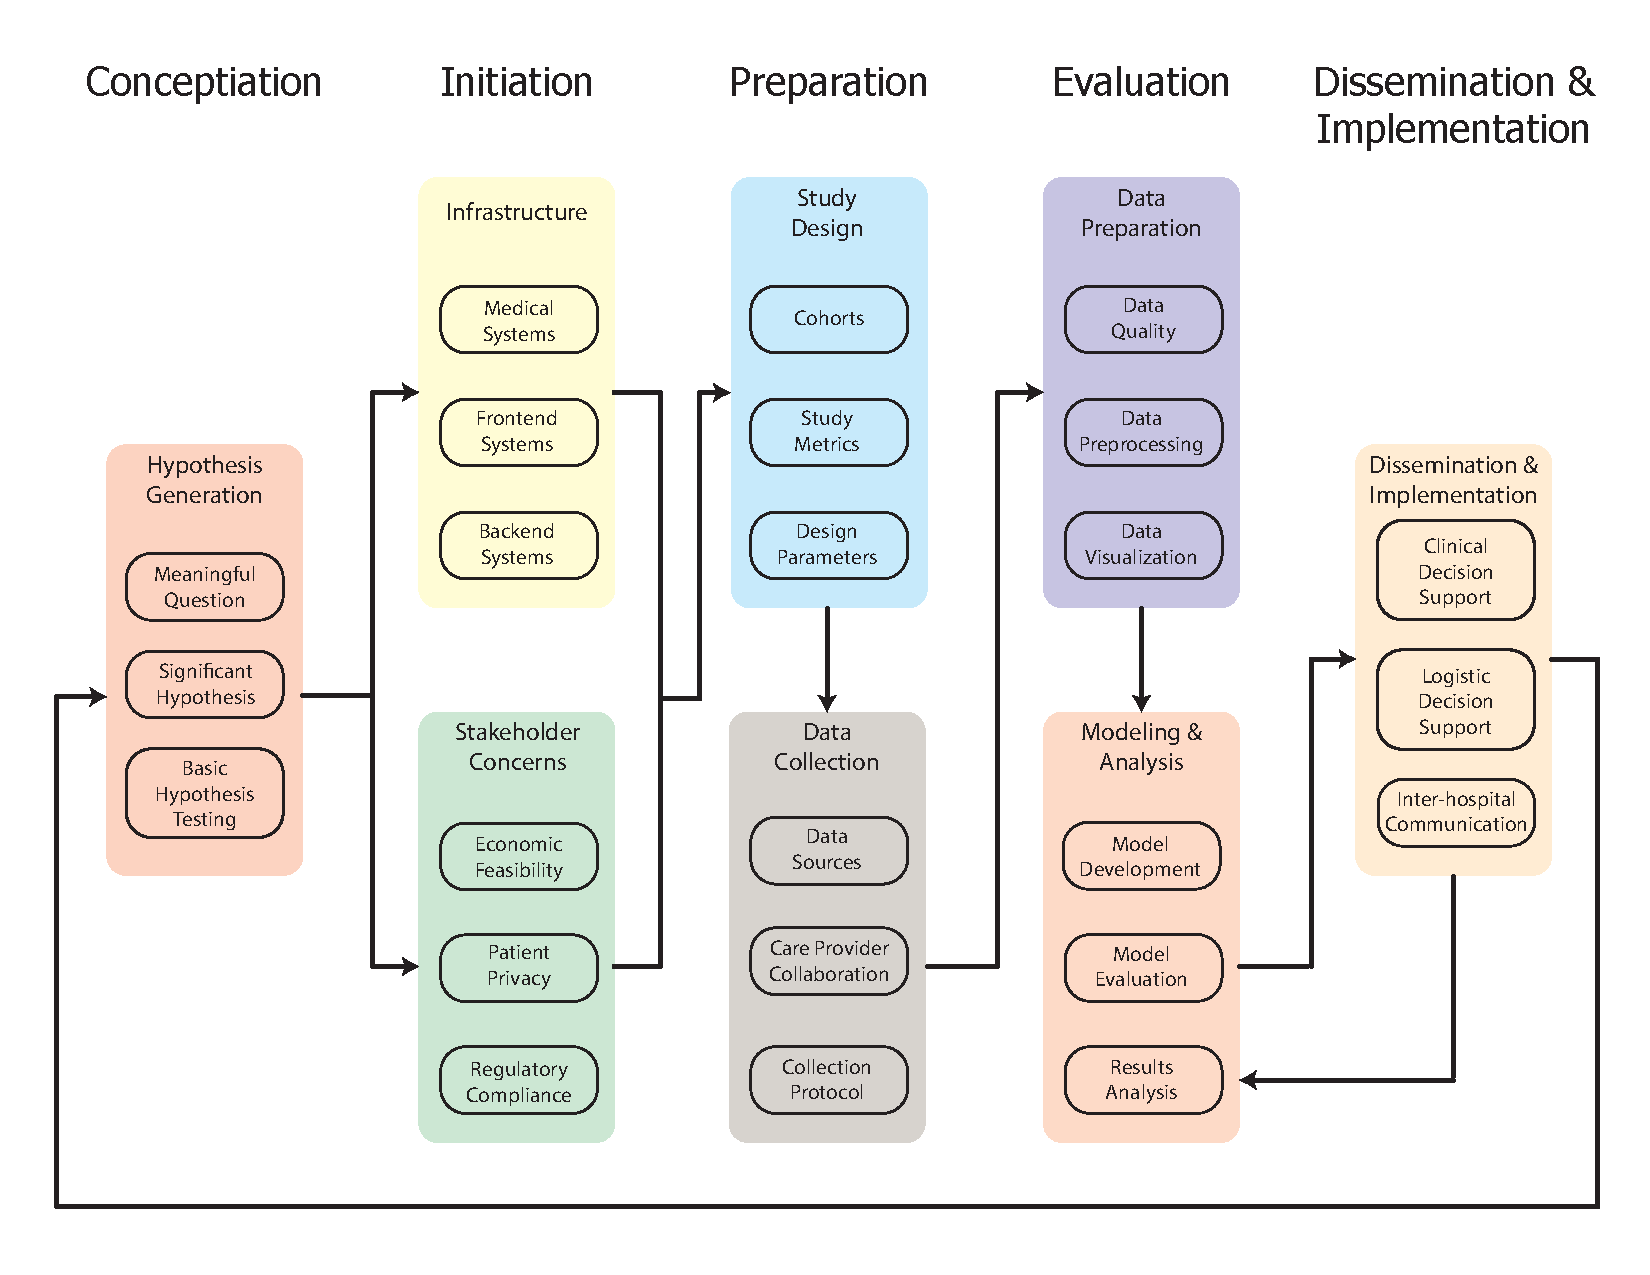
\includegraphics[width=0.8\textwidth]{images/informatics_pipeline.pdf}	
	\end{center}
\end{frame}





\end{document}